%!TEX root = ../Hardtung_BA_SoSe20.tex

\section{Virtual Folding of the Paper}
\label{sec:virtualFolding}

When creating diagrams with the Origrammer, the most time-consuming activity is the placement of all required lines. All edges, current creases, and existing creases have to be placed precicely to allow the user to closely follow the instructions simply by the visual cues. This large bottleneck in the diagramming process can only be eliminated by simulating the actual folding process virtually.

Being able to drag and drop a corner or edge of the paper to the desired position would significantly reduce the work required.

 \begin{figure}[htbp]
	\centering
	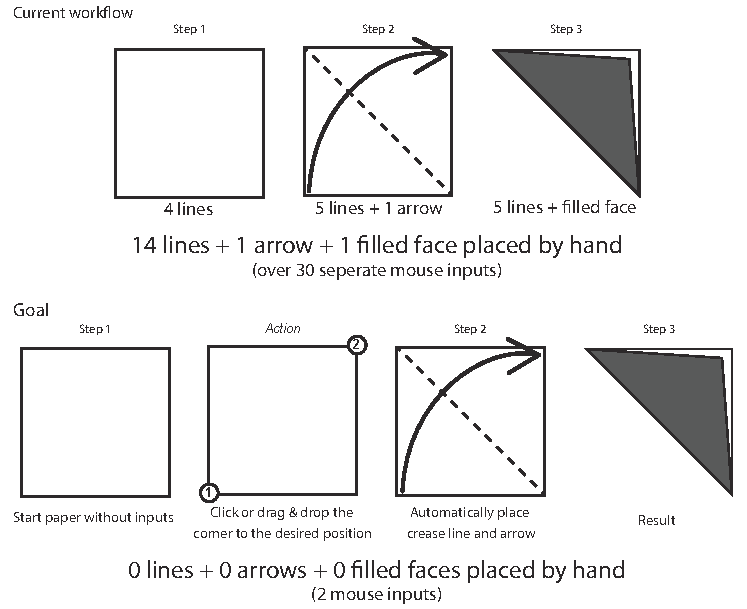
\includegraphics[width=\textwidth]{virtualFoldingGoal}
	\caption{Current workflow (top) \& Desired workflow (bottom)}
	\label{fig:virtualFoldingGoal}
\end{figure}

\noindent To implement this automated folding, several parts of the Origrammer will have to be reworked. As there have already been a few attempts to simulate paper folding, the following sections will explore these projects to gain additional knowledge relevant for the Origrammer rework.


\subsection{Related Works}
Folding virtually to simulate folding origami models constitutes a goal pursued by several projects. This section will list and explore several of those attempts to gain information on how the folding had been implemented in these projects. Building on this extant knowledge, the implementation of the Origrammer can be developed further while additionally improving on previous attempts at the same time.

\subsubsection{Origami Simulation}
\begin{figure}[htbp]
	\centering
	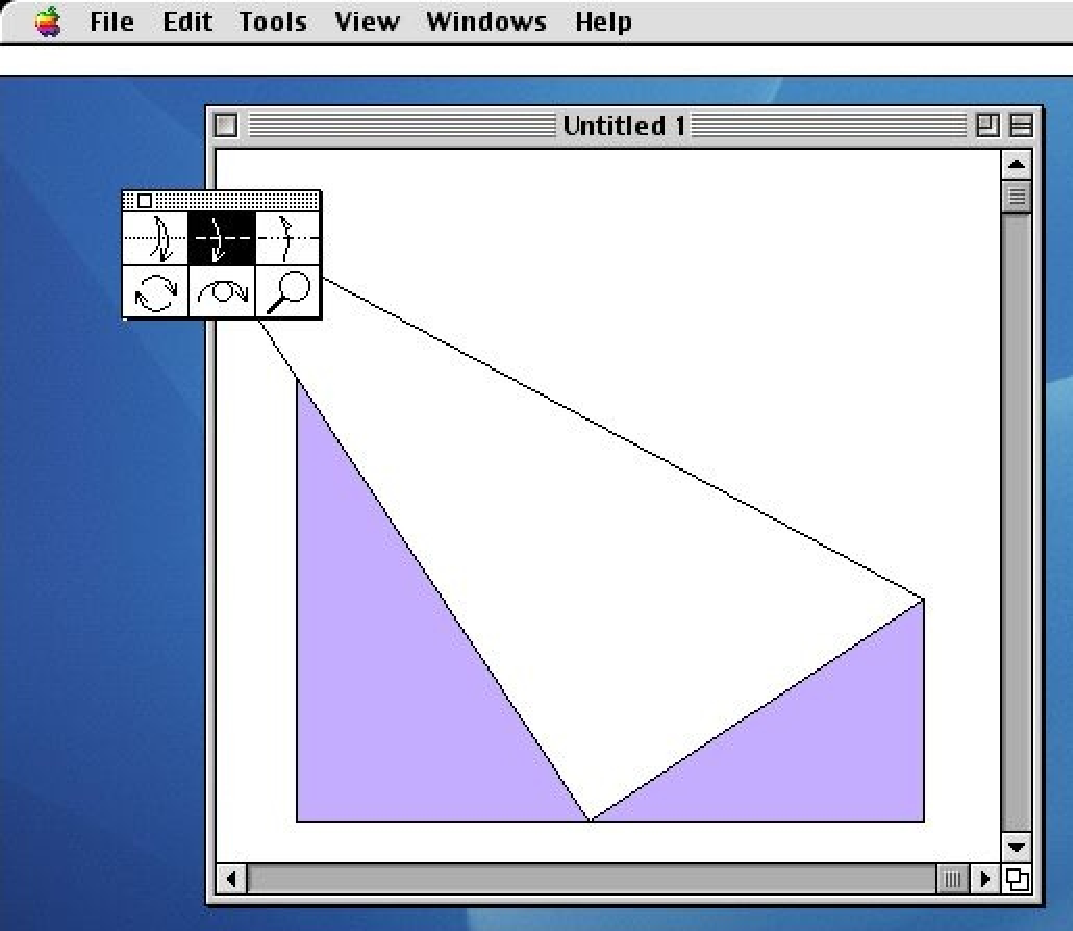
\includegraphics[width=0.63\textwidth]{origamiSimulation}
	\caption{Origami Simulation by Robert J. Lang}
	\label{fig:origamiSimulation}
\end{figure}
\noindent One of the first documented approaches to simulate origami folding is \emph{Origami Simulation} \cite{origamiSimulation} by Robert J. Lang. This desktop application was ``written in Object Pascal for the Mac OS, using Lightspeed's THINK Pascal and the THINK Class Library'' (Lang, 2015, para. 2 \cite{origamiSimulation}) . It is able to carry out simple Valley and Mountain Folds, as well as to rotate and turn the paper around.
Though, as this application was originally developed in the 1980s, it is now only runnable on Mac Classic mode, such that it does no longer run on Mac OS X 10.5 and later or on Intel-based Macs. However, the source code is still publicly available\footnote{\url{http://www.langorigami.com/wp-content/uploads/2015/09/origamisim.src_.zip}} and could prove useful for conceptional purposes when implementing the virtual folding of the Origrammer.

\subsubsection{Foldinator}
 \begin{figure}[htbp]
	\centering
	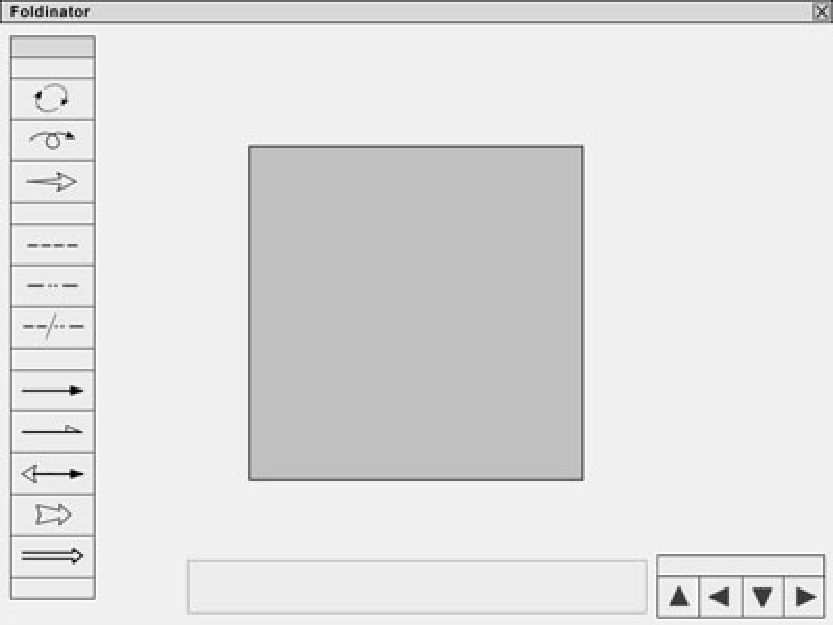
\includegraphics[width=0.7\textwidth]{foldinator}
	\caption{Foldinator by John Szinger}
	\label{fig:foldinator}
\end{figure}

\noindent The Foldinator \cite{foldinator} is a software application developed by John Szinger aiming at virtualizing the folding process and subsequently creating origami diagrams.
The program was originally developed in Flash using ActionScript1 but was later ported to the Apache Flex SDK\footnote{\url{http://flex.apache.org/index.html}}. The paper in Szingers approach was represented by polygons that are split up and moved when folding. Further, there is no puplicly available explanation on what constraints and processes are used for the folding itself.

Featurewise, the Foldinator is able to carry out Valley and Mountain folds, rotate, and turn the paper around.

\newpage
\subsubsection{eGami}
\label {eGami}
 \begin{figure}[htbp]
	\centering
	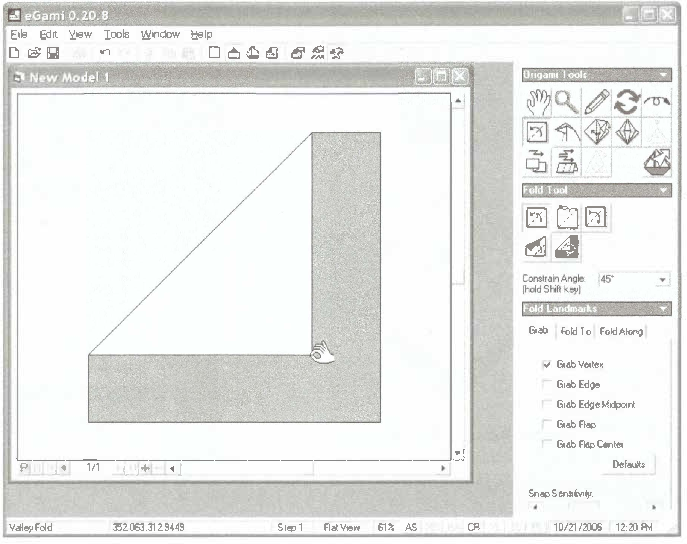
\includegraphics[width=0.9\textwidth]{eGami}
	\caption{eGami by Jack Fastag}
	\label{fig:eGami}
\end{figure}
\noindent The desktop application eGami \cite{eGami} by Jack Fastag can simulate the folding of flat origami models and create automatically generated diagrams. While publicly available information on which programming language the application was developed on could not be identified, the paper published in \emph{Origami\textsuperscript{4}: Fourth International Meeting of Origami Science, Mathematics, and Education} contains more detailed explanations of the inner workings.

eGami is using a winged-edge boundary representation (Foley, 1996, p.545-546 \cite{wingedEdge}) to store and work with a polygon mesh, which is representing the paper. Through this representation, a series of constraints ensures correct properties of the paper. Additional constraints also guarantee that only valid folds can be carried out:

\setstretch{0.5}
\begin{minipage}{10cm}
\begin{center}
\begin{enumerate}[label=(\alph*)]
\item{\emph{All polygons are closed}}
\item{\emph{All edges are used by not more than two polygons}}
\item{\emph{Each vertex is referenced by at least two edges and at least one polygon}}
\item{\emph{The mesh is completely connected, topologically planar and has no holes}}
\item{\emph{Vertices on the raw edge of the paper must be connected to exactly two ``raw'' edges}}
\item{\emph{Vertices inside the paper must satisfy Maekawa's Theorem}}
\item{\emph{Paper does not stretch, which means vertex positions are fixed and edge lengths are constant}}
\item{\emph{Paper faces are flat, which means that each polygon's vertices are coplanaer and implies that only rigid folds are allowed}}
\item{\emph{No rips or holes}}
\item{\emph{Paper is infinitely thin, implying that paper ``creep'' is not taken into account}}
\item{\emph{Only flat folds are allowed, meaning each vertex inside the paper must satisfy Kawasaki's Theorem}}
\item{\emph{Paper does not intersect itself}}\\
\end{enumerate}
\end{center}
\end{minipage}
\onehalfspacing
\newline
(Fastag, 2006, 3.1 \cite{eGami})\\


\noindent Implementation of Maekawa's and Kawasaki's theorems of flat foldability\cite{hull1994mathematics} in addition to the other mentioned constraints could improve the reliability of Origrammer's virtual folding and should be pursued further.

\subsubsection{Conclusion}

\noindent Previous attempts at virtually folding paper for diagram creation have proven its viability. Unfortunately, they have either not been updated in years or never proceeded further than simple Valley and Mountain folds. Additionally, for most projects there is no detailed information available on how these programs work and how they actually implement the folding simulations. So for the Origrammer, all underlying processes should be explained and documented. This will give a starting point for other future approaches to the virtual folding. Furthermore, a set of constraints (similar to eGami \ref{eGami}) should be implemented ensuring that only valid folds can be made.

\newpage
\subsection{Requirements}

The following aspects build the concrete requirements of what the virtual folding should do automatically and what has to be kept track of in order to implement this system of simulated folding.

The paper lines have to be stored in a way such that their relations and connections to each other are stored and preserved. Then, as seen in Figure \ref{fig:virtualFoldingGoal}, the folding arrows have to be placed automatically when folding parts of the paper. The folding line where the new crease is created should be placed automatically, as well. This crease line might also have to go through multiple layers of paper, which will have to be checked for each folding action. Lastly, the folded part of the paper has to actually change position and direction, and possibly show the differently colored side of the paper.

\subsection{Current Status}

So far, every line got stored within a single \texttt{ArrayList<OriLine>} and was otherwise completely independent of the other lines. An additional\\
\texttt{ArrayList<OriVertex>} is tracked to efficiently iterate through all vertices that can be used as an input point for new lines, arrows, or symbols. All arrows and symbols got also stored within their respective \texttt{ArrayList<>} per folding step. Lastly, the folding steps themselves got stored within an \texttt{ArrayList<Step>} as well, thereby, making the saving of the full diagram in a .xml-file simple and efficient.

This approach worked reliably while there were no dependencies between the lines and vertices. But when folding virtually, several dependencies and other values have to be tracked. These include the edge lines, existing creases, newly made creases (all with their specific line types), correct layering when rendering folded paper, correct colouring of different paper sides, and the rendering with slight distortions to show hidden layers/flaps (Lang, 2011, para. \emph{Distort the model to show all the layers} \cite{Lang}), among others.

\newpage
\subsection{Reworked System}

The new implementation works by splitting the actual paper model into \texttt{OriPolygons} that can be folded, split up, and rendered (see Listing \ref{oriPolygon}).
\begin{lstlisting}[label=oriPolygon,caption=OriPolygon]
OriPolygon {
        OriVertexList vertexList; 
        ArrayList<OriLine> lines;
        int height; /*height of the polygon (rendering order)*/
}
\end{lstlisting}

\noindent Once the user inserts a new fold line, the Origrammer checks which \texttt{OriPolygons} are affected by the fold and subsequently splits them at the points where the folding line crosses the edges of a given polygon. The resulting line at the newly created crease is now a shared line between the two smaller, split up polygons. This is more closely visualized at Figure \ref{fig:reworkedPaperRepresentation}.
 \begin{figure}[htbp]
	\centering
	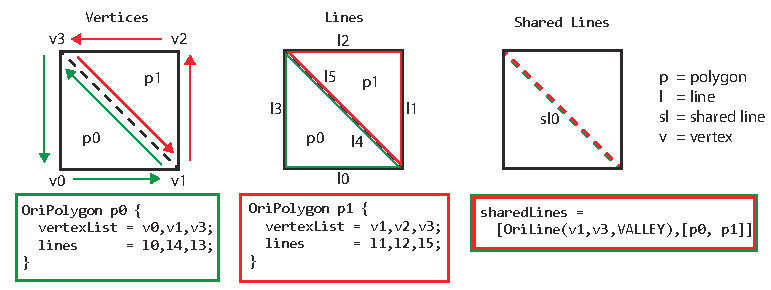
\includegraphics[width=\textwidth]{reworkedPaperRepresentation}
	\caption{Reworked Paper Representation through \texttt{OriPolygons} and \texttt{sharedLines}}
	\label{fig:reworkedPaperRepresentation}
\end{figure}

\noindent Every \texttt{OriPolygon} in turn consists of a \texttt{OriVertexList}, which contains all vertices of aforementioned polygon in a counter-clockwise order. Additionally, an \texttt{ArrayList<OriLine>} is required to keep track of the edge lines of the paper. As an \texttt{OriLine} also includes the line type, the lines within the \texttt{OriPolygon.lines}-list can have the type \texttt{EDGE} or \texttt{SHARED}.

For the case that a polygon is sharing a line with another polygon, the \texttt{HashMap<OriLine, ArrayList<OriPolygon>> sharedLines} was added.

\begin{lstlisting}[label=paperModelImplementation,caption=New Implementation of Paper Model]
ArrayList<OriPolygon> polygons

HashMap<OriLine, <ArrayList<OriPolygon>> sharedLines
\end{lstlisting}

\noindent This \emph{shared lines}-list contains all the shared lines in combination of which polygons are sharing the given line. Additionally, the real line type is stored here, which is later used for rendering. If the \texttt{OriPolygons} stored the actual line type instead of the mockup type \texttt{SHARED}, then there is no programmable connection between several \texttt{OriPolygons}. This would make folding lines that go through multiple polygons at the same time harder to calculate and progress.

Alternatively, there could be a flag for each \texttt{OriLine} that would signalize if it is also a shared line. But then one would have to iterate through all \texttt{OriPolygons} and check each individual line in them when looking for the connected polygon of a given shared line. So even though the \texttt{HashMap} of shared lines has to be updated and kept track of at all times, it is still more flexible and efficient compared to the system of flagging an \texttt{OriLine} as a shared line.

\begin{lstlisting}[label=oriVertexList,caption={OriVertexList, OriVertex, and OriLine}]
OriVertexList {
        int n; /*vertex count*/
        OriVertex head;
}

OriVertex {
        Vector2d p; /*Vector2d(x, y)*/
        OriVertex prev;
        OriVertex next;
}

OriLine {
        OriVertex p0;
        OriVertex p1;
        int type; 
        /*NONE, EDGE, MOUNTAIN, VALLEY, XRAY, CREASE, 
        (SHARED), (DIAGONAL)*/
}
\end{lstlisting}

\newpage

 \begin{figure}[htbp]
	\centering
	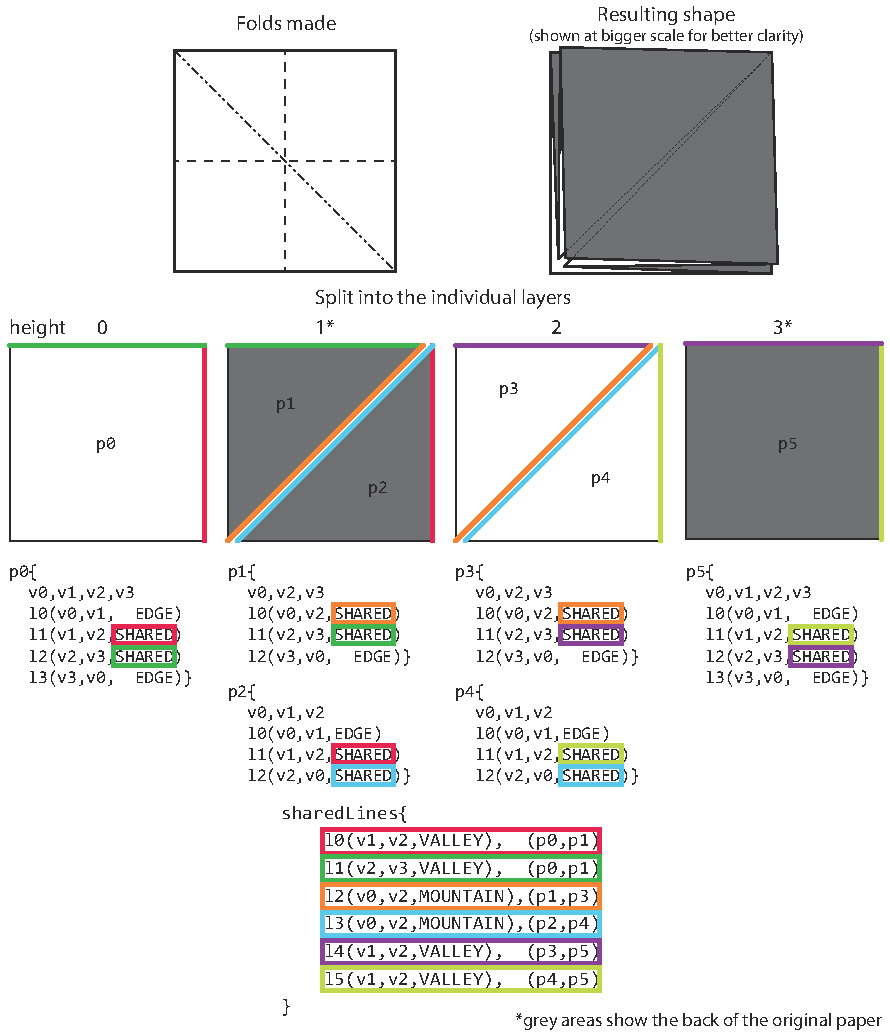
\includegraphics[width=\textwidth]{complexVirtualFolding}
	\caption{A more complex example of splitting polygons and multiple layers}
	\label{fig:complexVirtualFolding}
\end{figure}

\noindent The example in Figure \ref{fig:complexVirtualFolding} shows a slightly more complex example how the Origrammer splits the polygons and creates the correct shared lines. Additionally, in this case multiple layers of the paper have to be rendererd and kept track of. This height value is only preserved for each \texttt{OriPolygon} and is not used in the vertices, lines, or shared lines. It appears worth highlighting that for each shared line there can only be two \texttt{OriPolygon}s that share one edge. So when making a fold on one polygon and this fold crosses a shared line of this polygon, the Origrammer only has to search for the counterpart polygon, that shares the same line. This process can be seen in Figure \ref{fig:heightValuesWhenFolding}, where a fold through multiple layers is carried out. Internally, the Origrammer starts with a simple folding line on the top polygon that goes to its edges. If one or both endpoints of the folding line end in a shared line, it is clear that other polygons are also affected by this fold. Then one has to only iterate through the list of shared lines and find the connected polygon/s. Once the new \texttt{OriPolygon}/s have been found, the same process can be repeated subsequently.


\begin{enumerate}
\item Create the folding line on the top layer
\item Check both endpoints if they are ending in a shared line
\item Find the connected polygons on the sides that have a shared line
\item Repeat step 1-3 with the next highest layer until on layer 0 or no other polygons are found
\end{enumerate}

\begin{figure}[htbp]
	\centering
	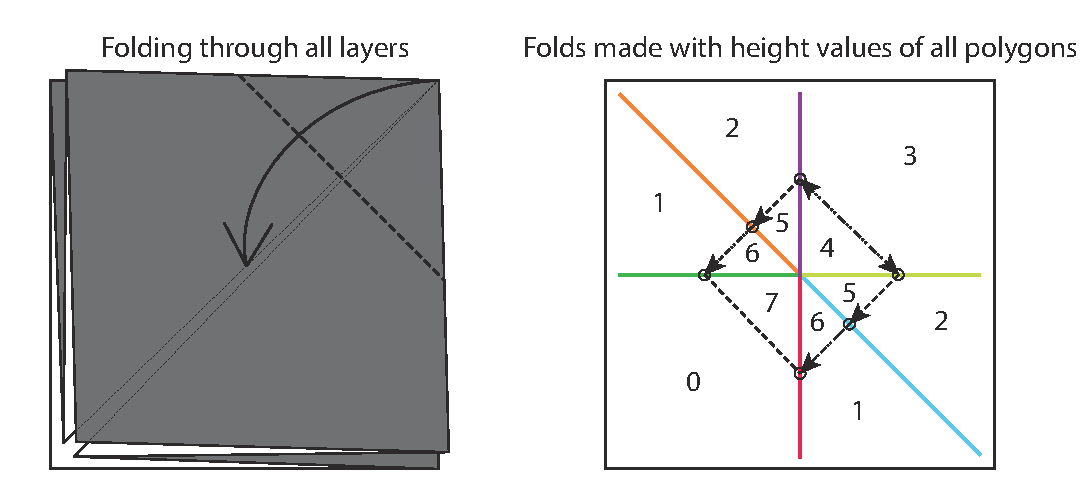
\includegraphics[width=\textwidth]{heightValuesWhenFolding}
	\caption{The process of folding through multiple layers and the updated height values}
	\label{fig:heightValuesWhenFolding}
\end{figure}

\noindent Figure \ref{fig:heightValuesWhenFolding} additionally highlights that the colored lines (shared lines) will have to be splilt up when applying the mountain and valley folds. The marked crease lines also represent newly made shared lines, as they split existing polygons.

%\begin{figure}[htbp]
%	\centering
%	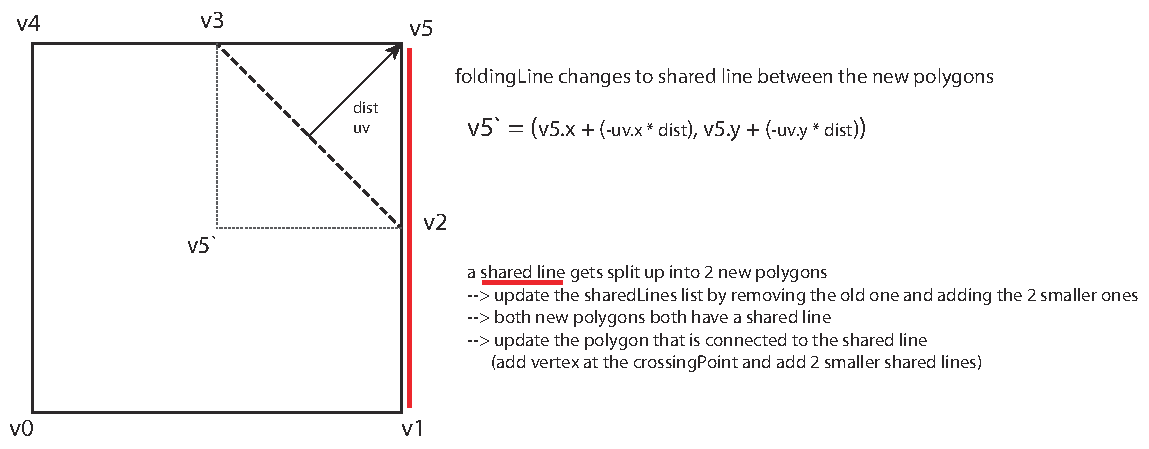
\includegraphics[width=\textwidth]{updatingVerticesWhenFolding}
%	\caption{Process of updating the new vertex positions after folding and splitting existing shared lines}
%	\label{fig:updatingVerticesWhenFolding}
%\end{figure}

\newpage
\subsubsection{Current Limitations}
\label{sec:virtualFoldingLimits}

The current implementation of the virtual folding still inherently contains limitations. While the user can freely fold the paper, even through multiple layers and in different directions, several more complex folding procedures can - yet -  not be carried out.

\subsubsection*{Reverse Folds}
Reverse Folds allow the paper to change directions. Inside Reverse Folds are made when pushing a corner of two layers in between these layers. At the same time, the original folding line between the two layers is being reversed, which explains the origin of its name.
\begin{figure*}[htbp]
	\centering
	\begin{subfigure}{0.4\textwidth}
		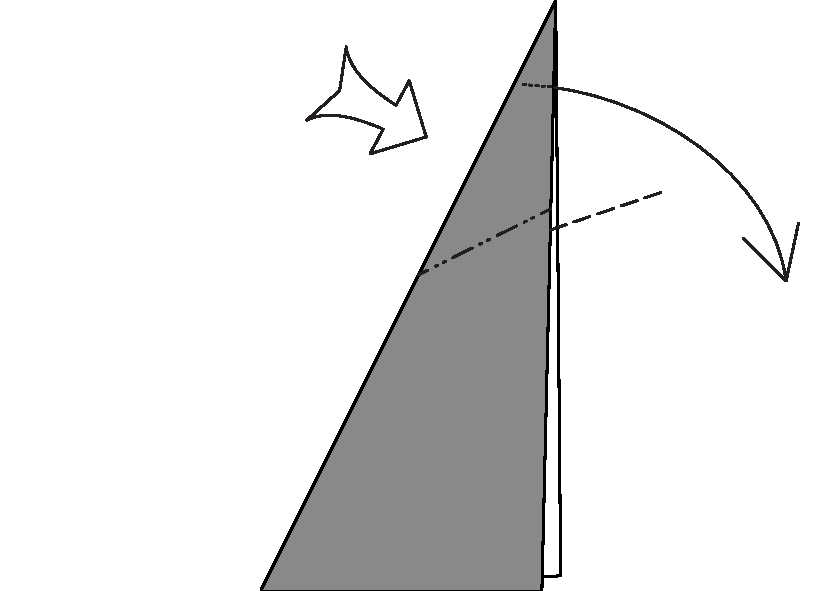
\includegraphics[width=\textwidth]{InsideReverseFold}
		\caption{Folding Action}
		\label{fig:insideReverseFoldA}
	\end{subfigure}
	\begin{subfigure}{0.4\textwidth}
		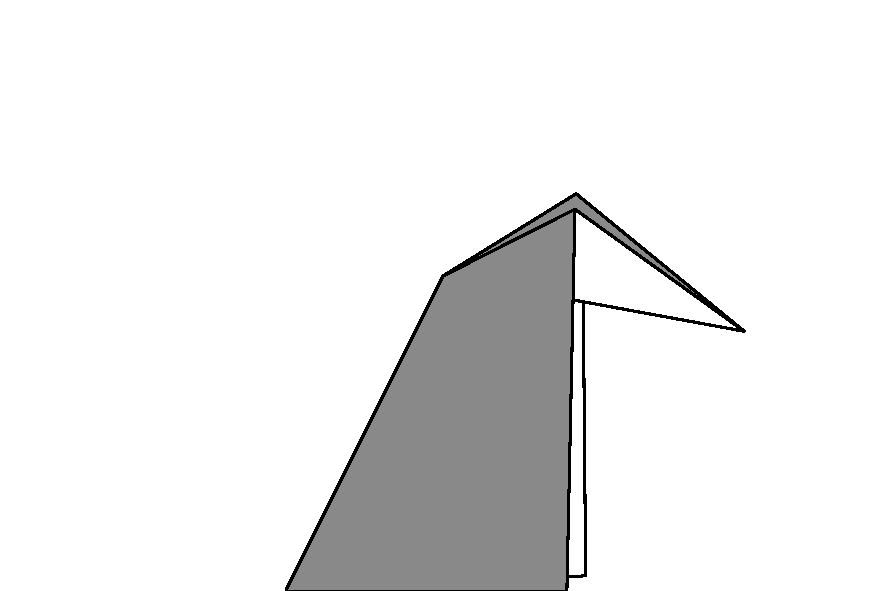
\includegraphics[width=\textwidth]{InsideReverseFoldResult}
		\caption{Result}
		\label{fig:insideReverseFoldResult}
	\end{subfigure}
	\caption{Inside Reverse Fold}
	\label{fig:insideReverseFold}
\end{figure*}


\noindent While for Inside Reverse Folds the paper is sunken into the layers of the paper, for Outside Reverse Folds, the fold wraps over the paper.
\begin{figure*}[htbp]
	\centering
	\begin{subfigure}{0.3\textwidth}
		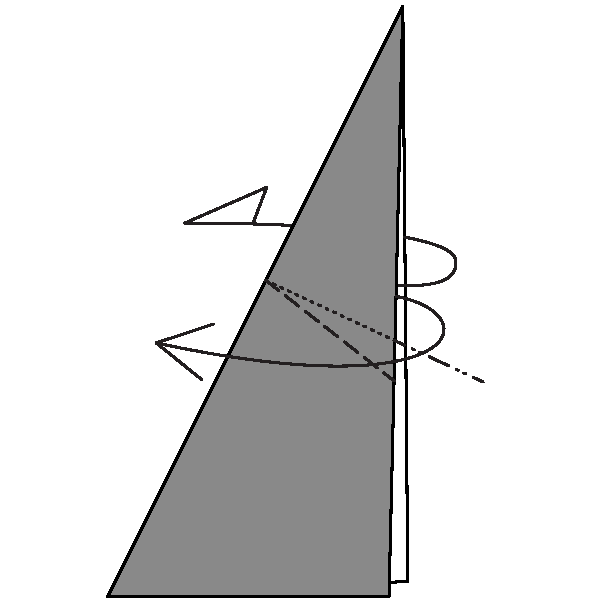
\includegraphics[width=\textwidth]{OutsideReverseFoldB}
		\caption{Folding Action}
		\label{fig:outsideReverseFoldB}
	\end{subfigure}
	\begin{subfigure}{0.3\textwidth}
		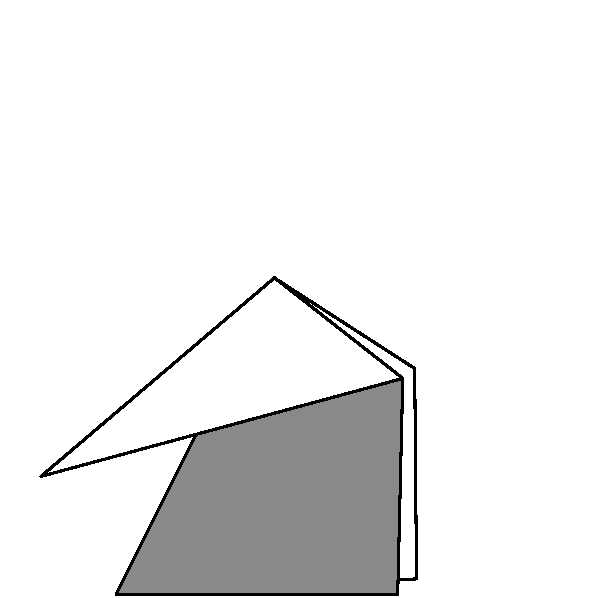
\includegraphics[width=\textwidth]{OutsideReverseFoldResult}
		\caption{Result}
		\label{fig:outsideReverseFoldResult}
	\end{subfigure}
	\caption{Outside Reverse Fold}
	\label{fig:outsideReverseFold}
\end{figure*}

\noindent The Reverse Folds require a mountain as well as a valley fold at the same time, while also changing the height values of the affected layers. As the Origrammer can currently only carry out one fold at a time, it can not make Reverse Folds yet.

\subsubsection*{Pleating and Crimping}

Pleats can be created by the Origrammer, as the folding process only requires two different, independent folds (see Fig. \ref{fig:pleating}). As these folds don't intersect or affect each other, they can be carried out one by one. Though this folding procedure could still be made more straight forward by offering a specific function for pleats. This way the user would only have to create one instead of two seperate folding actions.
\begin{figure*}[htbp]
	\centering
	\begin{subfigure}{0.49\textwidth}
		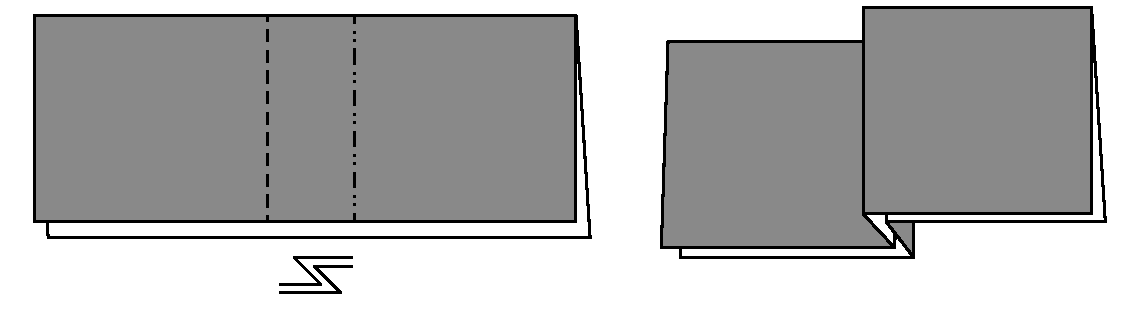
\includegraphics[width=\textwidth]{Pleating}
		\caption{Pleat}
		\label{fig:pleating}
	\end{subfigure}
	\begin{subfigure}{0.49\textwidth}
		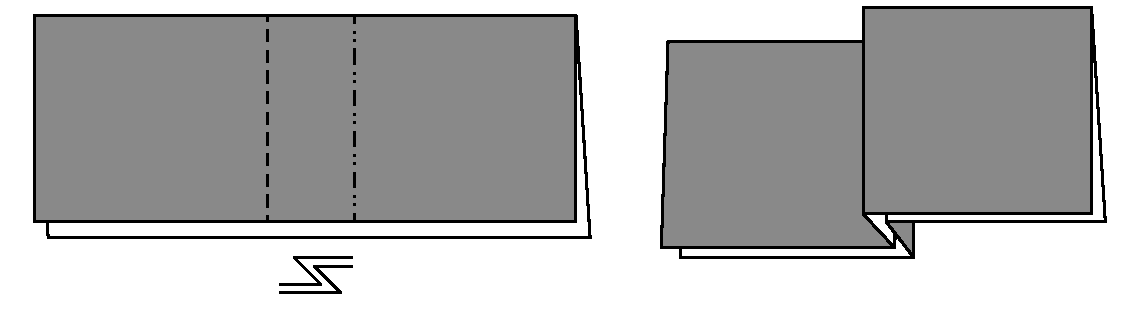
\includegraphics[width=\textwidth]{Crimping}
		\caption{Crimp}
		\label{fig:crimping}
	\end{subfigure}
	\caption{Pleats and Crimps}
\end{figure*}

\noindent Crimps on the other hand require one additional step. They can be started by a simple pleat followed by immediately folding it in half, thereby, creating a crimp. It needs to be highlighted that one part of the crimp partially encapsulates the other side. This can be seen in Fig. \ref{fig:crimping} where the right part of the paper surrounds the left. Even though a crimp could technically already be carried out by the Origrammer in three seperate steps, it is desirable to create a dedicated crimp-feature. This is especially important when the paper is already folded in half and a crimp has to be folded from there. Folding a crimp in this vein is currently not possible as the Origrammer would have to carry out two mountain and two valley folds at the same time.

\subsubsection*{Sinks}

The most complex folding procedures to automatically carry out by the Origrammer are the so-called sinks. The examples in Fig. \ref{fig:sinks} show the three different types, the open, the mixed, and the closed sink. A basic open sink is performed by pushing a corner of paper (with multiple layers) downwards and reversing the direction of all folds within the pushed-in corner at the same time. This reversing of existing creases is visualized in the so-called \gls{creasePattern} from Fig. \ref{fig:sinks}. A crease pattern displays an unfolded view of the paper, but still shows all existing mountain and valley folds. Through this approach, even the hidden creases can be shown to give a full overview.\\
But as the crease patterns show, multiple existing crease lines have to be reversed and almost all height values of the layers change, as well. This makes the calculations for the automated folding more complex - especially when sinking multiple layers at the same time.
\begin{figure}[htbp]
	\centering
	\begin{subfigure}{\textwidth}
		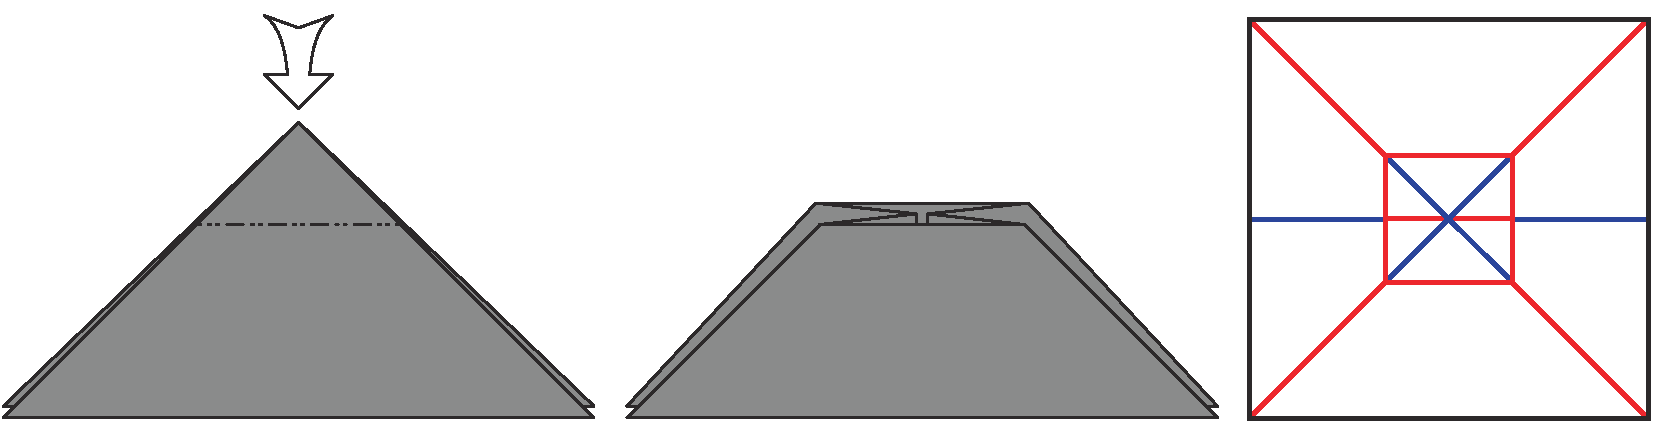
\includegraphics[width=0.9\textwidth]{OpenSink}
		\caption{Open Sink}
		\label{fig:openSink}
	\end{subfigure}
	\begin{subfigure}{\textwidth}
		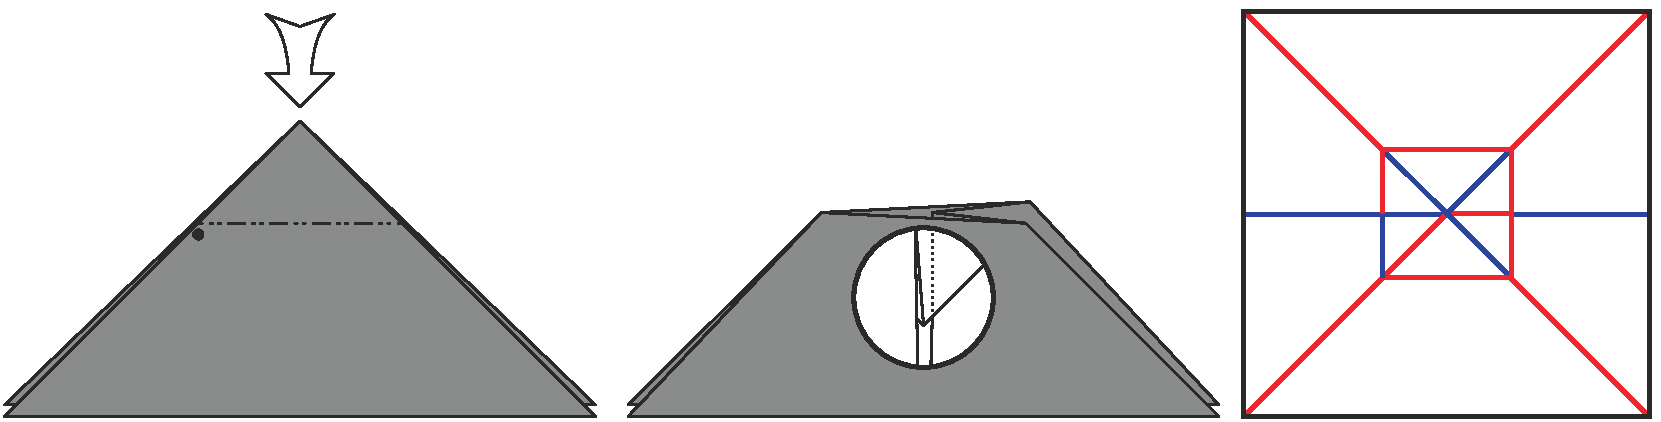
\includegraphics[width=0.9\textwidth]{MixedSink}
		\caption{Mixed Sink}
		\label{fig:mixedSink}
	\end{subfigure}
	\begin{subfigure}{\textwidth}
		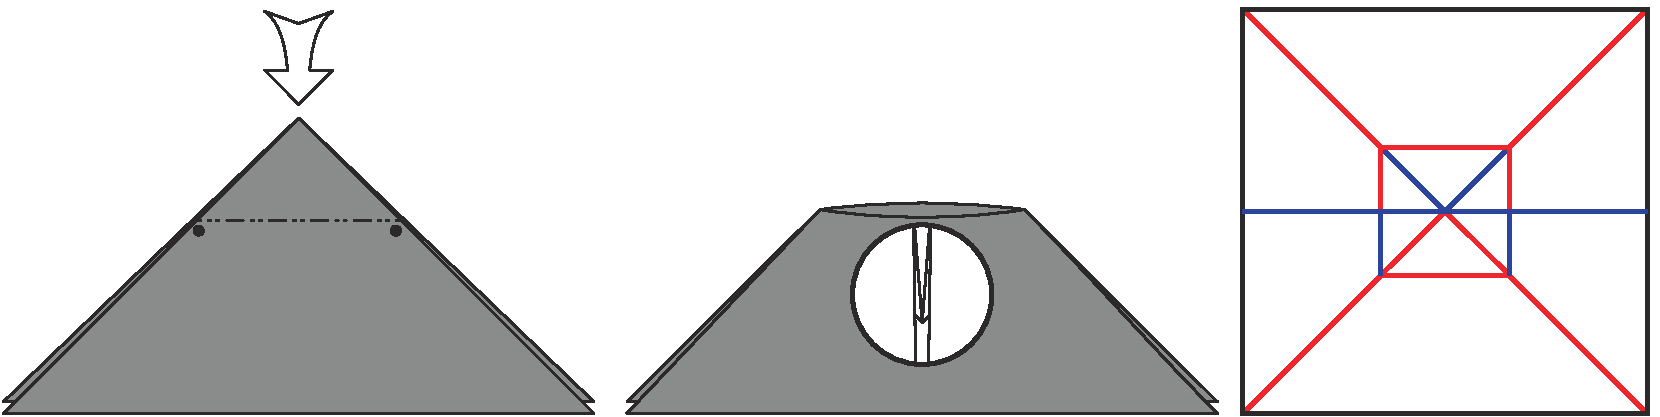
\includegraphics[width=0.9\textwidth]{ClosedSink}
		\caption{Closed Sink}
		\label{fig:closedSink}
	\end{subfigure}
	\begin{subfigure}{\textwidth}
	        \centering
		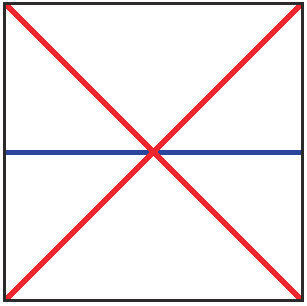
\includegraphics[width=0.23\textwidth]{sinkPreCP}
		\caption{Crease Pattern before creating a Sink}
		\label{fig:sinkPreCP}
	\end{subfigure}
	\caption[Different forms of Sinks]{Different forms of Sinks\footnotemark}
	\label{fig:sinks}
\end{figure}

\footnotetext{red lines = mountain folds; blue lines = valley folds}
